\section{Computation of the Mandelbrot Set}

\begin{figure}[tb]
  \centering
  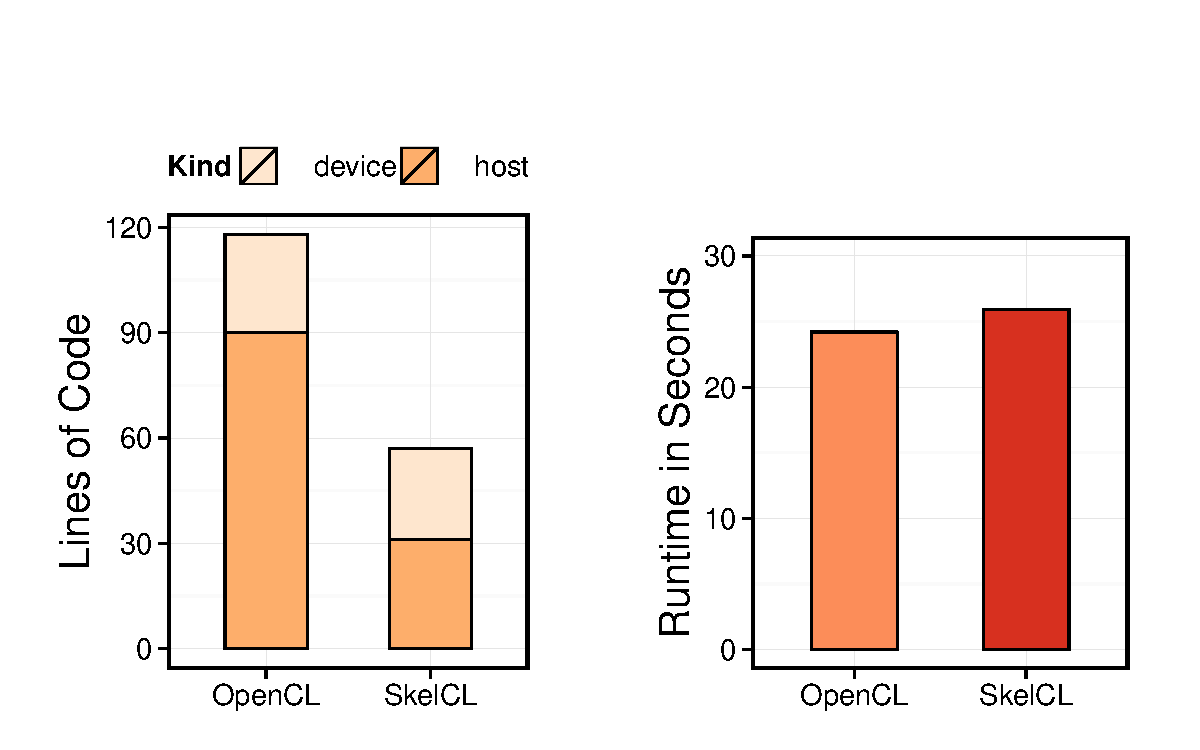
\includegraphics[width=.75\textwidth]{mandelbrot}
  \caption[Visualization of a part of the Mandelbrot set.]%
          {Visualization of a part of the Mandelbrot set. The image was produced using the \SkelCL library.}
  \label{fig:mandelbrot}
\end{figure}

The Mandelbrot~\cite{Mandelbrot1980} set includes all complex numbers $c \in {\mathbb C}$ for which the sequence
\begin{equation}
	z_{i+1} = z_{i}^{2} + c,\qquad i\in {\mathbb N}
	\label{eq:mandelbrot}
\end{equation}
starting with $z_{0}=0$ does not escape to infinity.
When drawn as an image with each pixel representing a complex number, the boundary of the Mandelbrot set forms a fractal.
\autoref{fig:mandelbrot} shows an image visualizing part of the Mandelbrot set.
The software producing the image was implemented using the \SkelCL library. 
The calculation of such an image is a time-consuming task, because the sequence given by~\autoref{eq:mandelbrot} has to be calculated for every pixel.
If this sequence does not cross a given threshold for a given number of iteration steps, it is presumed that the sequence will converge.
The respective pixel is thus taken as a member of the Mandelbrot set, and it is displayed black.
Other pixels outside are assigned a color that corresponds to the number of iterations of the sequence given by~\autoref{eq:mandelbrot}.
Computing a Mandelbrot fractal is easily parallelizable, as all pixels of the fractal can be computed simultaneously.

\subsubsection*{\SkelCL Implementation}
\label{sec:mandelbrot:implementation}
The Mandelbrot set computations expressed in the \SkelCL programming model uses the \map skeleton as shown in \autoref{eq:skelcl:mandelbrot}.
\begin{align}
  mandelbrot\ w\ h =&  \nonumber\\
         map\ compute&ColorOfPixel\ (generateIndex\ w\ h)
  \label{eq:skelcl:mandelbrot}
\end{align}
% \todo{Explain $generateIndex$ and connection to \ref{eq:mandelbrot}}
Here function $mandelbrot$ is defined taking two arguments -- the width $w$ and height $h$ of the image to compute.
The function is defined in terms of the \map skeleton which is customized with the $computeColorOfPixel$ function computing the color of a single pixel of the image (not shown here) and operating on an input matrix of size $w\times h$ consisting of indices.
This input matrix is generated by the $generateIndex$ function which -- given a width $w$ and height $h$ -- produces a matrix containing all combinations of pairs $(x,y)$ of indices $x$ and $y$ with $x < w$ and $y < h$.

The implementation of the Mandelbrot set computation using the \SkelCL library is shown in \autoref{lst:skelcl:mandelbrot}.
A user-defined data type is introduced to represent the color of a pixel (line~\ref{lst:skelcl:mandelbrot:pixel}).
An instance of the \map skeleton is created in line~\ref{lst:skelcl:mandelbrot:map} and applied to \code{IndexMatrix} (line~\ref{lst:skelcl:mandelbrot:apply}).
The \code{IndexMatrix} represents all indices up to a given width and height.
It is implemented as a special representation of the more generic \code{Matrix} class avoiding the explicit storing of the indices in memory.
Instead when accessing an element the index value is computed on the fly.
This implementation avoids allocation of memory for storing the indices and transferring them to the \GPU.


\begin{lstlisting}[%                                                             
caption={Implementation of the Mandelbrot set computation in \SkelCL},%
numbers=left,%
float=tb,
label={lst:skelcl:mandelbrot}]
typedef struct { char r; char g; char b; } Pixel;$\label{lst:skelcl:mandelbrot:pixel}$

Pixel computeColorOfPixel(IndexPoint) { ... };

void mandelbrot(const int width, const int height) {
  auto m = map(computeColorOfPixel);$\label{lst:skelcl:mandelbrot:map}$
  auto image = m(IndexMatrix{w, h});$\label{lst:skelcl:mandelbrot:apply}$
  writeToDisk(image); }
\end{lstlisting}

We created a similar parallel implementations for computing a Mandelbrot fractal using OpenCL.
We compare the programming effort and performance for these implementations against our \SkelCL implementation.

\subsubsection*{Programming effort}
\label{sec:mandelbrot:programming}

\SkelCL require a single line of code for initialization in the host code, whereas OpenCL requires a lengthy initialization of different data structures which takes about 20 lines of code.

The host code differs significantly between both implementations.
In OpenCL, several API functions are called to load and build the kernel, pass arguments to it and to launch it using a specified work-group size.
In \SkelCL, the \map skeleton is used to compute the color of all pixels in the image.
An \code{IndexMatrix} representing complex numbers, each of which is processed to produce a pixel of the Mandelbrot fractal, is passed to the \map skeleton upon execution.
Specifying the work-group size is mandatory in OpenCL, whereas this is optional in \SkelCL.

\paragraph{Program size}
The OpenCL-based implementation has 118 lines of code (kernel: 28~lines, host program: 90~lines) and is thus more than twice as long as the \SkelCL versions with 57 lines (26, 31) (see \autoref{fig:mandelbrot_runtime}).

\paragraph{Kernel size}
The kernel function is similar in both implementations: it takes a pixel's position (\ie, a complex number) as input, performs the iterative calculation for this pixel, and returns the pixel's color.
However, while the input positions are given explicitly when using the \map skeleton in SkelCL, no positions are passed to the kernel in the OpenCL-based implementation.
The positions are implicitly determined based on the work-item's index.

\subsubsection*{Performance experiments}
\label{sec:mandelbrot:performance}

\begin{figure}[tb]
    \centering
    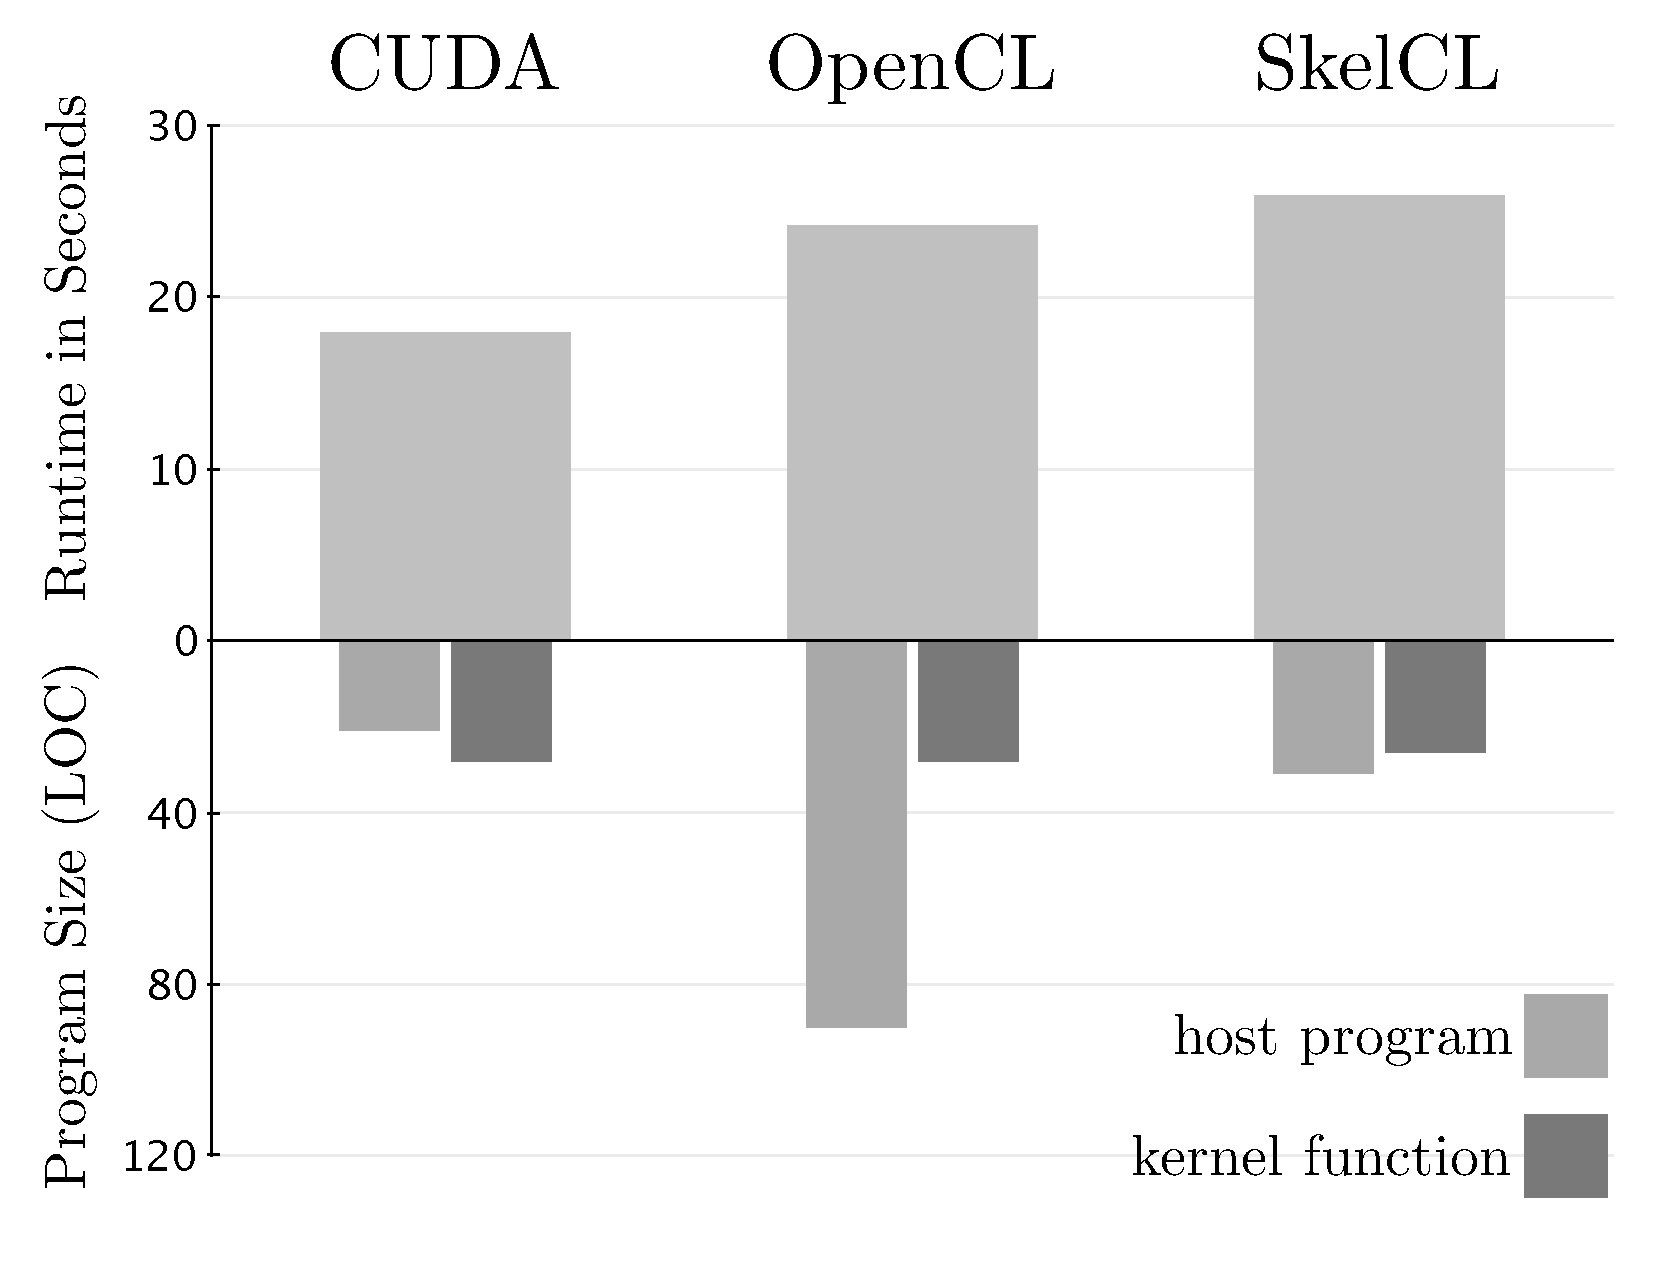
\includegraphics[width=0.6\textwidth]{HIPS/ChartMandelbrot}
    \caption{Runtime and program size of the Mandelbrot application.}
    \label{fig:mandelbrot_runtime}
\end{figure}%


We tested our implementations on a single \GPU of our test system to compute a Mandelbrot fractal of size 4096$\times$3072 pixels.
In OpenCL, work-groups of 16$\times$16 are used; \SkelCL uses its default work-group size of~256 work-items.

The results are shown in \autoref{fig:mandelbrot_runtime}.
As compared to the runtime of the \SkelCL-based implementation (26 seconds), the implementation based on OpenCL (25 seconds) is faster by 4\%.
Since \SkelCL is built on top of OpenCL, the performance difference of \SkelCL and OpenCL can be regarded as the overhead introduced by SkelCL.
% Previous work~\cite{KongDiYaLiCaStMaZh2010} also reported that CUDA was usually faster than OpenCL, which also explains the higher performance of the implementation based on CUDA.
The Mandelbrot application demonstrates that \SkelCL introduces a tolerable overhead of less than 5\% as compared to OpenCL.
A clear benefit of this overhead is the reduced programming effort required by the SkelCL program.

